\chapter{Αλγόριθμος Black-Scholes}
\label{chap:black_scholes}

\section{Εισαγωγή}
\begin{frame}
  \frametitle{Εισαγωγή}
  \begin{itemize}
    \item Ο αλγόριθμος Black-Scholes είναι ένα μοντέλο για την τιμολόγηση ευρωπαϊκών δικαιωμάτων προαίρεσης.
    \item Ο αλγόριθμος αυτός αναπτύχθηκε το 1973 από τους Fischer Black, Myron Scholes και Robert Merton.
    \item Η εξίσωση Black-Scholes είναι μια διαφορική εξίσωση που περιγράφει την εξέλιξη της τιμής ενός δικαιώματος προαίρεσης με την πάροδο του χρόνου.
  \end{itemize}

  \begin{block}{Σημαντικότητα}
    \begin{itemize}
      \item Ο αλγόριθμος Black-Scholes έχει επηρεάσει σημαντικά την ανάπτυξη των χρηματοοικονομικών αγορών.
      \item Έχει κερδίσει το βραβείο Νόμπελ Οικονομίας το 1997 για την εφαρμογή του στη χρηματοοικονομική θεωρία.
    \end{itemize}
  \end{block}
\end{frame}

\section{Αλγόριθμος Black Scholes}

H εξίσωση του μοντέλου θεωρεί ότι μέσα όπως μετοχές ή συμβόλαια μελλοντικής εκπλήρωση:
\begin{itemize}
    \item θα έχουν μια λογαριθμοκανονική κατανομή των τιμών
    \item θα ακολουθεί έναν τυχαίο περίπατο με σταθερή μετατόπιση και μεταβλητότητα.
\end{itemize}

Η εξίσωση χρησιμοποιεί αυτή την υπόθεση και συνυπολογίζει άλλες σημαντικές μεταβλητές για να προκύψει η τιμή ενός δικαιώματος αγοράς ευρωπαϊκού τύπου.

Το μοντέλο Black-Scholes απαιτεί τις πέντε μεταβλητές που αναλύθηκαν προηγουμένως:
\begin{itemize}
    \item την τιμή άσκησης ενός δικαιώματος προαίρεσης
    \item την τρέχουσα τιμή της μετοχής
    \item το χρόνο μέχρι τη λήξη
    \item το επιτόκιο χωρίς κίνδυνο
    \item και τη μεταβλητότητα.
\end{itemize}

Επίσης περεταίρω παραδοχές που πρέπει να αναφερθούν είναι:

\begin{itemize}
    \item Η τιμή του υποκείμενου περιουσιακού στοιχείου ακολουθεί γεωμετρική κίνηση Brownian (αλλιως διαδικασία Wiener) η οποία περιγράφεται απο την εξίσωση:
    \begin{equation}
      dS = \mu S\,dt + \sigma S\,dW
    \end{equation}
    Οπου $W$ είναι μια τυχαία μεταβλητή που ακολουθεί κανονική κατανομή.
    Εχει μέση τιμή 0 και διασπορά $\sigma^2t$.
    \begin{figure}[H]
      \centering
      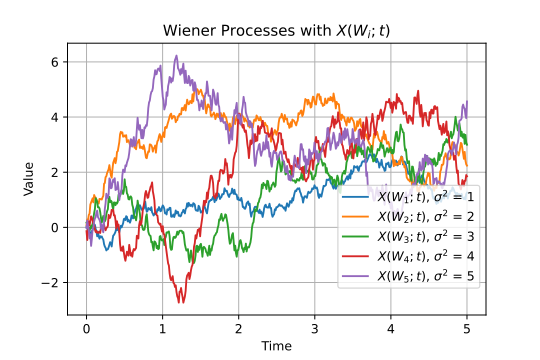
\includegraphics[width=1.0\textwidth]{./figures/chapter2/wiener_process.png}
      \caption{Γραφική απεικόνιση της γεωμετρικής κίνησης Brownian}
      \label{fig:black_scholes_brownian}
    \end{figure}
    \item Κατά τη διάρκεια της διάρκειας του δικαιώματος προαίρεσης δεν καταβάλλονται μερίσματα.
    \item Οι αγορές είναι τυχαίες επειδή οι κινήσεις της αγοράς δεν μπορούν να προβλεφθούν.
    \item Δεν υπάρχουν έξοδα συναλλαγής κατά την αγορά του δικαιώματος προαίρεσης.
    \item Το επιτόκιο χωρίς κίνδυνο και η μεταβλητότητα του υποκείμενου περιουσιακού στοιχείου είναι γνωστά και σταθερά.
    \begin{tcolorbox}[colframe=blue!50!black, colback=blue!5, title=Ορισμός Προαιρεσης Μετοχών]
        Η μεταβλητότητα στην πραγματικότητα δέν ειναι σταθερή και είναι συνάρητηση του χρόνου μέχρι την λήξη και την τιμή  του δικαιώματος προαίρεσης.
        \begin{figure}[H]
          \centering
          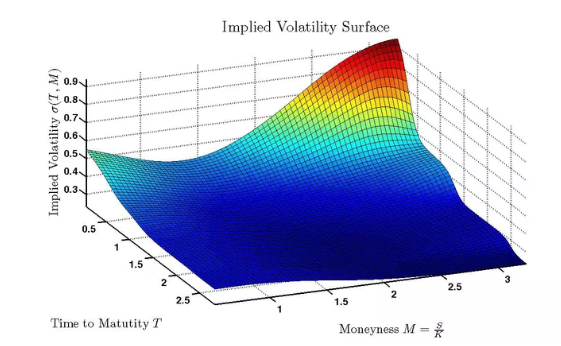
\includegraphics[width=1.0\textwidth]{./figures/chapter2/volatility_surface.png}
          \caption{Τρισδιάστατη απεικόνιση της επιφάνειας μεταβλητότητας}
          \label{fig:volatility_surface}
        \end{figure}
        Τα κύρια χαρακτηριστικά της επιφάνειας μεταβλητότητας είναι ότι τα δικαιώματα προαίρεσης με χαμηλότερες τιμές άσκησης τείνουν 
        να έχουν υψηλότερες μεταβλητότητες. Για μια δεδομένη λήξη $T$, αυτό το χαρακτηριστικό αναφέρεται συνήθως ως "volatility skew" ή "volatility smile".
        Για μια δεδομένη τιμή άσκησης $K$, η μεταβλητότητα μπορεί είτε να αυξάνεται είτε να μειώνεται με τον χρόνο μέχρι τη λήξη.
        Σε γενικές γραμμές, όμως, η $\sigma(K, T)$ τείνει να συγκλίνει σε μια σταθερά καθώς ο χρόνος μέχρι την λήξη τείνει στο άπειρο $T \to \infty$. 
        Για μικρές τιμές $T$, ωστόσο, συχνά παρατηρούμε μια αντεστραμμένη επιφάνεια μεταβλητότητας, με τα δικαιώματα προαίρεσης βραχυπρόθεσμης 
        λήξης να έχουν πολύ υψηλότερες μεταβλητότητες από τα μακροπρόθεσμα.
    \end{tcolorbox}
    \item Οι αποδόσεις του υποκείμενου περιουσιακού στοιχείου κατανέμονται κανονικά.
    \item Το δικαίωμα προαίρεσης είναι ευρωπαϊκό και μπορεί να ασκηθεί μόνο κατά τη λήξη.
\end{itemize}

Ο τύπος του Black-Scholes υπολογίζεται πολλαπλασιάζοντας την τιμή της μετοχής με τη συνάρτηση τυπικής κατανομής πιθανοτήτων. 
Η καθαρή παρούσα αξία (ΚΠΑ) της τιμής εξάσκησης πολλαπλασιαζόμενη με τη συσωρευτική τυπική κανονική κατανομή και αφαιρείται στη συνέχεια από την προκύπτουσα τιμή του προηγούμενου υπολογισμού.
Συμφωνα και με την βιβλιογραφία [\cite{wikipedia_black_scholes}, \cite{haugh_black_scholes_columbia}]:

\begin{equation}
    C = S_0 N(d_1) - X e^{-rT} N(d_2)
\end{equation}

όπου:
\begin{itemize}
    \item $C$: Η τιμή του δικαιώματος προαίρεσης
    \item $S_0$: Η τρέχουσα τιμή της μετοχής
    \item $X$: Η τιμή άσκησης του δικαιώματος προαίρεσης
    \item $r$: Το επιτόκιο χωρίς κίνδυνο
    \item $T$: Ο χρόνος μέχρι τη λήξη
    \item $N(d)$: Η συνάρτηση κατανομής κανονικής πιθανότητας
\end{itemize}

Τα $d_1$ και $d_2$ υπολογίζονται με τους παρακάτω τύπους:
\begin{equation}
    d_1 = \frac{\ln(\frac{S_0}{X}) + (r + \frac{\sigma^2}{2})T}{\sigma \sqrt{T}}
\end{equation}
\begin{equation}
    d_2 = d_1 - \sigma \sqrt{T}
\end{equation}

και το N(d) είναι η συνάρτηση κατανομής κανονικής πιθανότητας, που υπολογίζεται με τον παρακάτω τύπο:
\begin{equation}
    N(d) = \frac{1}{\sqrt{2\pi}} \int_{-\infty}^{d} e^{-\frac{x^2}{2}} dx
\end{equation}

Το πρώτο μισο της εξίσωσης δηλαδή το $S_0 N(d_1)$ είναι η εκτίμηση της τιμής ασκησης,
ενώ το δεύτερο μισό της εξίσωσης, $X e^{-rT} N(d_2)$, είναι η εκτίμηση της καθαρής παρούσας αξίας της τιμής άσκησης του δικαιώματος προαίρεσης.

\subsection{Σημασία της Θεωρίας}
Το μοντέλο Black-Scholes κατέχει μεγάλη σημασία στον οικονομικό χώρο διότι εισήγαγε μια αυστηρή μαθηματική προσέγγιση για την τιμολόγηση των δικαιωμάτων προαίρεσης,
επιτρέποντας στους επενδυτές και στους διαχειριστές κινδύνου να εκτιμήσουν με ακρίβεια την αξία αυτών των χρηματοοικονομικών εργαλείων.
Πριν από την ανάπτυξή του, η τιμολόγηση των options βασιζόταν κυρίως σε εμπειρικές μεθόδους ή σε υποκειμενικές εκτιμήσεις.

Η επαναστατικότητα του μοντέλου έγκειται στα εξής:
\begin{itemize}
    \item \textbf{Αυστηρή Θεωρητική Βάση:} Το μοντέλο βασίζεται σε θεμελιώδεις αρχές των μαθηματικών και της στατιστικής, όπως η κανονική κατανομή και η στοχαστική ανάλυση.
    \item \textbf{Απλοποίηση της Τιμολόγησης:} Παρέχει έναν απλό και πρακτικό τύπο για την τιμολόγηση των ευρωπαϊκών δικαιωμάτων προαίρεσης, μειώνοντας την πολυπλοκότητα της διαδικασίας.
    \item \textbf{Ενίσχυση της Αγοράς Παραγώγων:} Η εφαρμογή του μοντέλου συνέβαλε στην ανάπτυξη και την ωρίμανση της αγοράς παραγώγων, καθιστώντας την πιο διαφανή και αποτελεσματική.
    \item \textbf{Διαχείριση Κινδύνου:} Το μοντέλο επιτρέπει στους επενδυτές να αντισταθμίσουν κινδύνους (hedging) με μεγαλύτερη ακρίβεια, βελτιώνοντας τη στρατηγική τους.
    \item \textbf{Επιστημονική Αναγνώριση:} Η απονομή του Βραβείου Νόμπελ στους δημιουργούς του υπογραμμίζει τη σημασία του για τη χρηματοοικονομική επιστήμη.
\end{itemize}

Η εισαγωγή του μοντέλου Black-Scholes άλλαξε ριζικά τον τρόπο με τον οποίο οι αγορές αντιλαμβάνονται και διαχειρίζονται τα δικαιώματα προαίρεσης, καθιστώντας το ένα από τα πιο σημαντικά επιτεύγματα στη χρηματοοικονομική μηχανική.

\section{Εφαρμογές}
\begin{frame}
  \frametitle{Εφαρμογές}
  \begin{itemize}
    \item Ο αλγόριθμος Black-Scholes χρησιμοποιείται ευρέως για την τιμολόγηση δικαιωμάτων προαίρεσης σε χρηματοοικονομικές αγορές.
    \item Χρησιμοποιείται επίσης για τη διαχείριση κινδύνου και την εκτίμηση της μεταβλητότητας των υποκείμενων περιουσιακών στοιχείων.
    \item Ο αλγόριθμος έχει επηρεάσει τη χρηματοοικονομική θεωρία και πρακτική, οδηγώντας σε νέες στρατηγικές και προϊόντα.
  \end{itemize}
  \begin{block}{Σημαντικές εφαρμογές}
    \begin{itemize}
      \item Τιμολόγηση δικαιωμάτων προαίρεσης
      \item Διαχείριση κινδύνου
      \item Εκτίμηση μεταβλητότητας
    \end{itemize}
  \end{block}
  \begin{block}{Σημαντικά προϊόντα}
    \begin{itemize}
      \item Ευρωπαϊκά δικαιώματα προαίρεσης
      \item Αμερικανικά δικαιώματα προαίρεσης
      \item Δικαιώματα προαίρεσης σε μετοχές και δείκτες
    \end{itemize}
  \end{block}
\end{frame}
\section{Συμπεράσματα}
\begin{frame}
  \frametitle{Συμπεράσματα}
  \begin{itemize}
    \item Ο αλγόριθμος Black-Scholes είναι ένα σημαντικό εργαλείο για την τιμολόγηση δικαιωμάτων προαίρεσης.
    \item Έχει επηρεάσει τη χρηματοοικονομική θεωρία και πρακτική, οδηγώντας σε νέες στρατηγικές και προϊόντα.
    \item Η κατανόηση του αλγορίθμου είναι κρίσιμη για τη διαχείριση κινδύνου και την εκτίμηση της μεταβλητότητας των υποκείμενων περιουσιακών στοιχείων.
  \end{itemize}
  \begin{block}{Σημαντικά σημεία}
    \begin{itemize}
      \item Ο αλγόριθμος Black-Scholes είναι ένα σημαντικό εργαλείο για την τιμολόγηση δικαιωμάτων προαίρεσης.
      \item Έχει επηρεάσει τη χρηματοοικονομική θεωρία και πρακτική.
      \item Η κατανόηση του αλγορίθμου είναι κρίσιμη για τη διαχείριση κινδύνου.
    \end{itemize}
  \end{block}
  \begin{block}{Σημαντικές παρατηρήσεις}
    \begin{itemize}
      \item Ο αλγόριθμος Black-Scholes έχει περιορισμούς και υποθέσεις που πρέπει να ληφθούν υπόψη.
      \item Η εφαρμογή του αλγορίθμου απαιτεί προσεκτική ανάλυση των παραμέτρων και των συνθηκών της αγοράς.
    \end{itemize}
  \end{block}
\end{frame}
